\chapter{Fundamentação teórica}
\label{CAP2}


Neste capítulo são apresentadas algumas formas de construir um perfil de consumo energético de algoritmos implementados em sistemas embarcados com exemplos de casos de usos e algumas técnicas de calcular o consumo de energia de algoritmos. Por fim, é apresentada uma técnica de emulação de captura de energia detalhando suas especificidades.


\section{Sistemas embarcados}
 A enorme de evolução dos sistemas embarcados fez com que a sociedade se tornar, de certa forma, dependente deles. Um Sistema Embarcado pela sua natureza especialista, pode ter inúmeras aplicações (CHASE, 2007). Aplicações, essa que vão desde o setor automotivo até a medicina chegando até mesmo ao vestuário. O avanço da tecnologias, em especial as digitais, irá afetar profundamente todas as estruturas econômicas e sociais, talvez a mais impactante e pervasiva dessas tecnologias digitais seja
a internet das coisas, objeto de atenção prioritária de governos e da iniciativa privada pelo mundo inteiro (MAGRANI, 2018).  O IoT ainda deve crescer muito nos próximos anos como mostra graficamente a Figura 1 da IHS (2016).  
\begin{figure}[!ht]
\centering
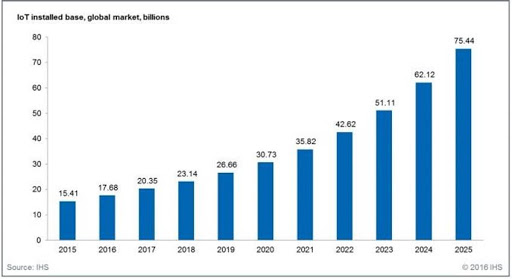
\includegraphics[scale=.65]{figures/grafico.jpg}
\caption{ Figura 1 - The IoT market will be massive. Fonte IHS (2016) } \label{Fig:1}
\end{figure}

Os avanços da microeletrônica proporcionaram o surgimento de diversos microprocessadores, microcontroladores, processadores de sinais digitais (DSP) e FPGA baseado em VLSI. Esse dispositivos estão presentes principalmente em dentro de outros dispositivos, sendo assim eles não são isíveis para o usuário ou seja são Ubíquos. Por seu baixo custo, desempenho satisfatório e em geral tamanho pequeno eles são sempre cotados para diversas aplicações. Não é atoa que os sistemas embarcados sejam os queridinhos do IoT, construir redes de comunicações inteiras entre dispositivos só se fez possível por causa deles. Eles também são responsaveis pelo processamento digital de divesos sinais.           



Cada um desses  microeletrônicos tem suas peculiaridades porém todos eles têm algo, muito nítido, em comum eles depende de energia para seu funcionando.Como estes sistemas são largamente usados em dispositivos que utilizam baterias como fonte de energia eles  devem ter consumo energético bastante restrito (NETO, et al. 2010). 
 Saber quanto é seu consumo energético se torna importante para seu total aproveitamento, uma parte desse consumo vem do algoritmo que está implementado no sistema. Para saber o consumo energético de determinados algoritmos existem alguns métodos que serão abordados a seguir.

\section{Métodos para calcular o consumo energético}

\subsection{Modelos Matematicos}
Construir um modelo matemático que possa determinar o desempenho energético um sistema sem que ele esteja montado fisicamente seria muito interessante, já que assim simplificaria e muito o processo de produção. Um modelo com essas características já foi construído para redes de sensores sem fio. O modelo proposto aborda uma parte importante do processo operacional das redes de sensores visuais sem fio, que é o processamento interno nos nós sensores (CERQUEIRA; COSTA, 2019).

\subsection{Simuladores}
Existem alguns simuladores de consumo energético um desse é o Sim-Panalyzer.  O SimpleScalar é um simulador de arquitetura computacional que modela um computador virtual com CPU, cache e hierarquia de memória e com base nesse modelo consegue simular programas reais executando sobre a plataforma especificada (LIMA; et al., 2012).

\subsection{Osciloscópio }
Dentre de todos os métodos relatados acima o osciloscópio é o mais tradicional quando se trata de medição de consumo de energia. Para a medição do consumo de energia foi usado o osciloscópio para medir a corrente consumida pelo processador ao executar o algoritmo desejado. Para medir a corrente, foi inserido um resistor de 0.333 Ohm conectado em série com o cabo de alimentação ATX12V da placa mãe e medida a diferença de voltagem da entrada e saída do resistor de shunt que foi inserido em série no circuito da placa principal,conforme se observa na Figura 2 ( NETO; MORENO; MATOS, 2011) .

\begin{figure}[!ht]
\centering
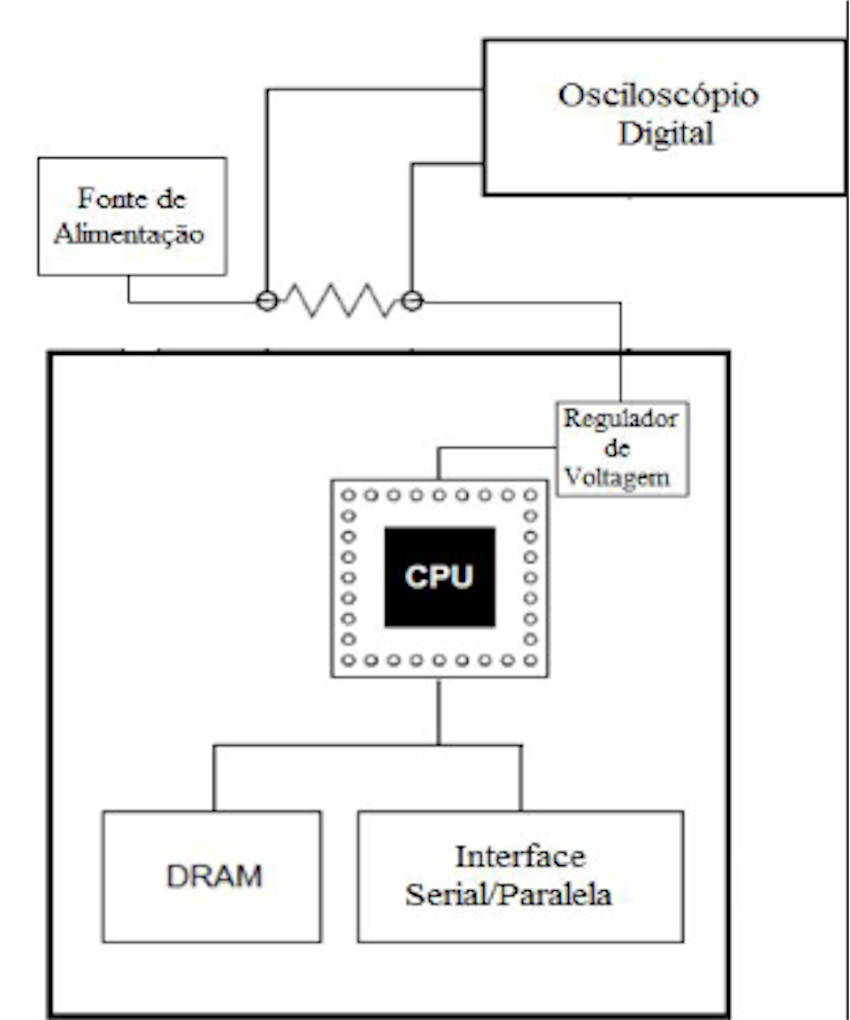
\includegraphics[scale=.65]{figures/ociloscopio.png}
\caption{ Figura 2 - Esquema utilizado para as medições com o Osciloscópio. Retirado de  ( Neto; Moreno; Matos, 2011). } \label{Fig:1}
\end{figure}


\section{Ripeto}
 Ripeto, uma plataforma de avaliação para EHES que pode imitar o comportamento do transdutor de captação de energia e registrar em rastreamentos de energia de memória e dados do analisador lógico para assegurar adequadamente o desempenho de um EHES (ALCANTARA; DE LIMA; FURTADO, 2019). O Ripeto é baseado em um FPGA Sparten6, da Xilinx, com 32 Mb de memória de DRAM acoplada.

\begin{figure}[!ht]
\centering
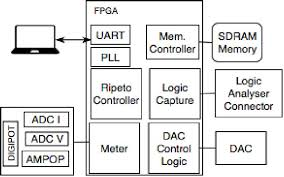
\includegraphics[scale=.65]{figures/ripeto.png}
\caption{Figura 3 - Arquitetura da Plataforma. Retirado de (ALCANTARA; DE LIMA; FURTADO, 2019) } \label{Fig:1}
\end{figure}

O elemento central, o FPGA é onde os  componentes lógicos são implementados. A intenção com essa plataforma é capturar os  perfis de fornecimento de energia de fontes renováveis e reproduzi los de forma consistente. O Ripeto é um excelente sistema embarcado para a realização dos experimentos deste trabalho, já que ele é uma plataforma embarcada com uma certa limitação energética. Sendo assim, ele foi escolhido para a realização dos experimentos do projeto.  
 

